\documentclass[aspectratio=169,14pt]{beamer}
\usetheme{TalentSprint}
\usepackage{caption}
\usepackage{csquotes}

\title[Regression Models]{Presentation Title} 

\begin{document}

{\1
\begin{frame}[plain,noframenumbering]
 \centerpage{Regression Models}
\end{frame}
}

\begin{frame}{A Simple Question}
\begin{overprint}
  \begin{itemize}
  \item<2->\alert{1, 3, 5, 7, 9, …	What is the next number?} \\
\uncover<3->{{\textcolor{tsgreen}{Ans:}} 11 - Odd numbers} \uncover<4->{\textcolor{red}{$2x+1$}}

\vspace{3ex}
\item<5-> \alert{1, 3, 9, 19, 33, ... What is the next number?} \\
 \uncover<6->{{\textcolor{tsgreen}{Ans:}} 51 }  \uncover<7->{\textcolor{red}{$2{x^2}+1$}}
  \end{itemize}
\end{overprint}
\end{frame}

\begin{frame}{A Simple Question}

\begin{block}{How do we solve such problems?}
\begin{itemize}
\item<2-> Find a pattern from the examples
\begin{itemize}
\item<2->(function \alert{$f(x)=2{x^2}+1$} or model the data)
\end{itemize}
\item<3-> Use it to predict the next number (or solve the  problem)
\end{itemize}
\end{block}
\uncover<4->{\alert{How do we design a computational procedure?}}
\end{frame}

\begin{frame}{A Simplified View of ML}
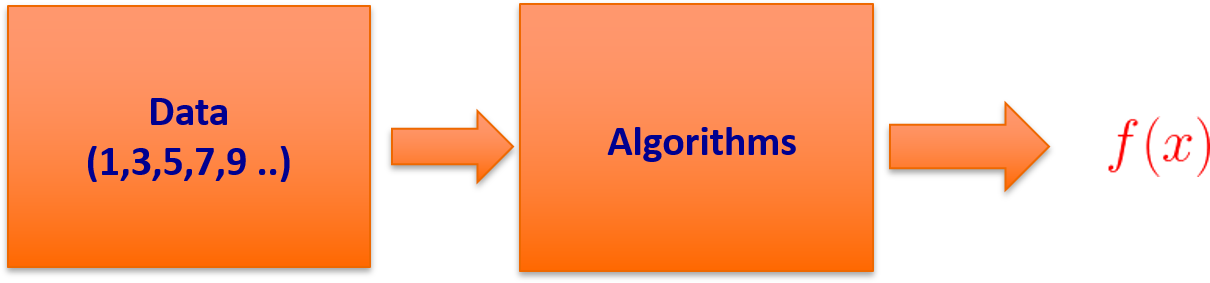
\includegraphics[width=13cm,height=3cm]{Images/Lin_reg_pic1.png}

\vfill
\hspace{8.8cm}
 $Eg:$ \\
\hfill
$int$  $function(int\;x[\hspace{1ex}])\{$ \\
\hspace{8.8cm}
$...$ \\
\hspace{8.8cm}
$\}$

\end{frame}


\begin{frame}{A Simple Question (Cont.)}
  \begin{itemize}
  \item<2->
 \alert{We know: 1, 3, 9, 19, 33, ... What is the next number?} \\
 \uncover<3->{{\textcolor{tsgreen}{Ans:}} 51 } \uncover<4->{{\textcolor{red}{$2{x^2}+1$}}}

\vspace{3ex}
\item<5->
\alert{0.99, 3.02, 9.00, 18.98, 33.01, ... What next?}
  \end{itemize}
\end{frame}

\begin{frame}{A Simple Question (Cont.)}
\begin{columns} 
\column{.5\textwidth}
\begin{overlayarea}{7cm}{5cm}
Consider a series of 2D points (1,3), (2,6), (3,9), (4,12), .... \\
\alert{What is the next point?}
\\~\\
\only<3>{\alert{($x,3x$)} or \\
The function: \alert{$y=f(x)=3x$}}
\end{overlayarea}


\column{.5\textwidth} 
\begin{overlayarea}{6.5cm}{4cm}
\includegraphics<2-2>[width=6.5cm,height=4cm]{Images/Lin_reg_Pic3.png}
\includegraphics<3-3>[width=6.5cm,height=4cm]{Images/Lin_reg_Pic2.png}
\end{overlayarea}
\end{columns} 
\end{frame}

\begin{frame}{What makes it Difficult?}
\uncover<2->{
	\begin{block}{When numbers are \enquote{uncertain}}
\begin{itemize}
\item Noise in measurements
\item Missing values
\end{itemize}
\end{block}}
\uncover<3->{
	\begin{block}{When numbers are not just \enquote{simple numbers}}
\begin{itemize}
\item 2D points, 3D points
\item 100 Dimensional points
\end{itemize}
\end{block}}
\end{frame}

\begin{frame}{Which line is Better (Fitting)?}
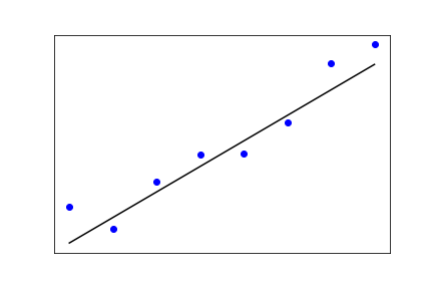
\includegraphics[width=6.5cm,height=4cm]{Images/Lin_reg_Pic4.png}
\hspace{3ex}
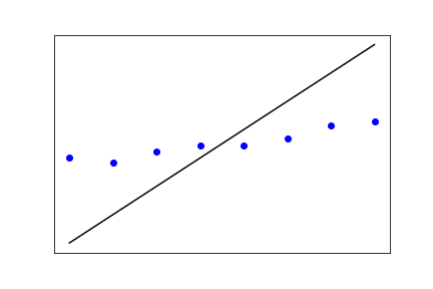
\includegraphics[width=6.5cm,height=4cm]{Images/Lin_reg_Pic5.png}
\end{frame}

\begin{frame}[t]{Which line is Better (Fitting)?}
\vspace{-0.8ex}
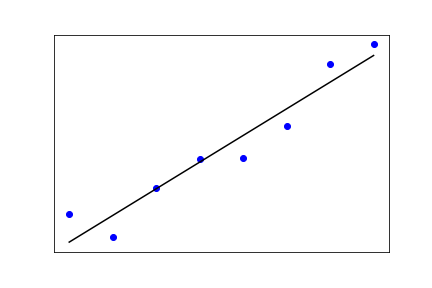
\includegraphics[width=3.5cm]{Images/Lin_reg_Pic6.png}    
\hfill
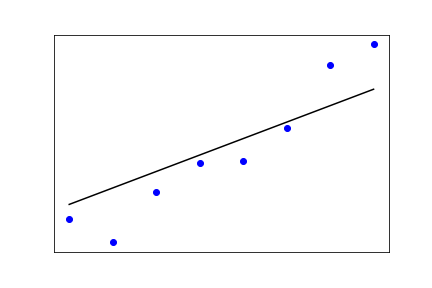
\includegraphics[width=3.5cm]{Images/Lin_reg_Pic7.png} \\
\vspace{-1ex}
\uncover<2->{\hspace{2ex}{\footnotesize W= (1.92, 1.71)}
\hspace{35.3ex}
{\footnotesize W= (1.15, 2.71)}} \\

\uncover<3->{\centering{\alert{How do we Decide?}}} \\
\vspace{-1ex}
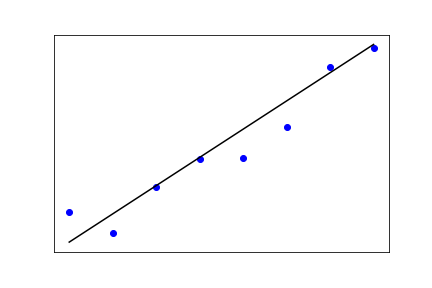
\includegraphics[width=3.5cm]{Images/Lin_reg_Pic8.png}    
\hfill
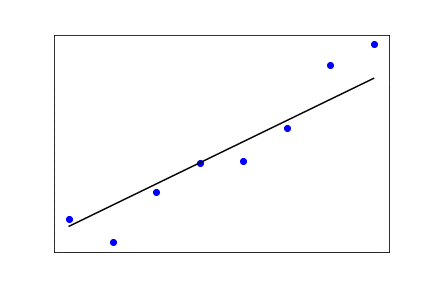
\includegraphics[width=3.5cm]{Images/Lin_reg_Pic9.png} \\
\vspace{-1ex}
\uncover<2->{\hspace{1.5ex}{\footnotesize W= (2.12, 2.91)}
\hspace{34.3ex}
{\footnotesize W= (1.48, 1.61)} }
\end{frame}

\begin{frame}[t]{Arrange in Descending Order of Error}
\vspace{-0.8ex}
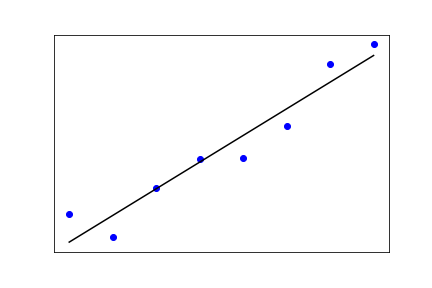
\includegraphics[width=3.5cm]{Images/Lin_reg_Pic6.png}    
\hfill
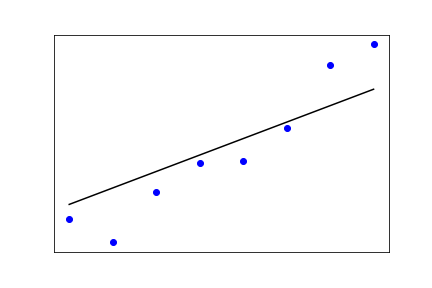
\includegraphics[width=3.5cm]{Images/Lin_reg_Pic7.png} \\
\vspace{-1ex}
\hspace{1.9ex}{\footnotesize W= (1.92, 1.71)}
\hspace{35.3ex}
{\footnotesize W= (1.15, 2.71)} \\

\vspace{-2ex}
\centering{\alert{Can we further decrease \\ the error metric chosen?}} \\

\vspace{-1.8ex}

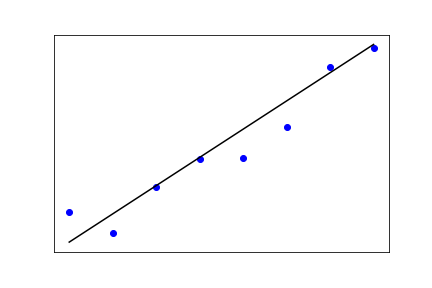
\includegraphics[width=3.5cm]{Images/Lin_reg_Pic8.png}    
\hfill
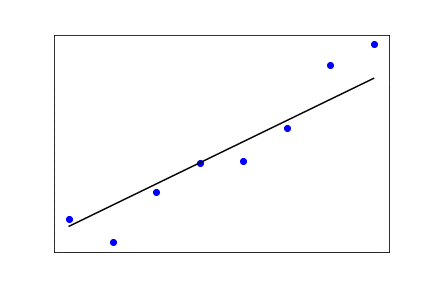
\includegraphics[width=3.5cm]{Images/Lin_reg_Pic9.png} \\
\vspace{-1ex}
\hspace{1.1ex}{\footnotesize W= (2.12, 2.91)}
\hspace{34.3ex}
{\footnotesize W= (1.48, 1.61)} 
\end{frame}

\begin{frame}{Looking Further}

\begin{itemize}
  \item<1-> Principle is to decrease the loss, say \alert{Mean Square error}
\item<1-> Iterative algorithms like Gradient descent for that purpose
\end{itemize}
\end{frame}


%\begin{frame}{Experiments}
%\begin{itemize}
%\item M0$\_$14$\_$Linearregression
%\item M0$\_$15$\_$Linearregression$\_$Diabetes
%\item M0$\_$16$\_$Linearregression
%\item M0$\_$17$\_$Linearregression$\_$HumanHeightWeight$\_$Human\\BrainWeightHeight$\_$BostonHousing
%\end{itemize}
%\end{frame}


\begin{frame}{Experiments}
\begin{itemize}
\item \href{https://drive.google.com/file/d/1lVRix6wwRteMKwwNGCofH-kFLkXDlPby/view?usp=sharing}{Demo\_Linear$\_$Regression$\_$Pendulumn}
\begin{itemize}
\item Dataset : Handmade dataset (where $L\propto T^2$)
\item Objective : To apply linear regression on the dataset
\end{itemize}
\item \href{https://drive.google.com/file/d/1JN_kUD4I1rX6ibho493PYo74jvuC-xs_/view?usp=sharing}{Demo\_Linearregression$\_$Diabetes}
\begin{itemize}
 \item Dataset : Diabetes
\item  Objective : To find the best fit line
\end{itemize}
\end{itemize}
\end{frame}



{\1
\begin{frame}[plain,noframenumbering]
 \centerpage{Thank you! \\ Questions?}
\end{frame}
}


\end{document}
